\subsubsection*{Kategorisering} \label{sec:kategorisering}
Første gang KOL-patienter logger ind i app'en, skal de foretage en individuel kategorisering. Dette er nødvendigt for at sikre, at brugeren får anbefalet et træningsniveau, som passer til deres helbred.
Kategoriseringen inddeler brugerne i A, B, C eller D, som beskrevet i \autoref{sec:klassifikation}. Af \autoref{fig:Kate} ses aktivitetsdiagrammet for kategoriseringen.

\begin{figure} [H]
\centering
\textbf{Aktivitetsdiagram: Kategorisering af KOL-patienter}\par\medskip
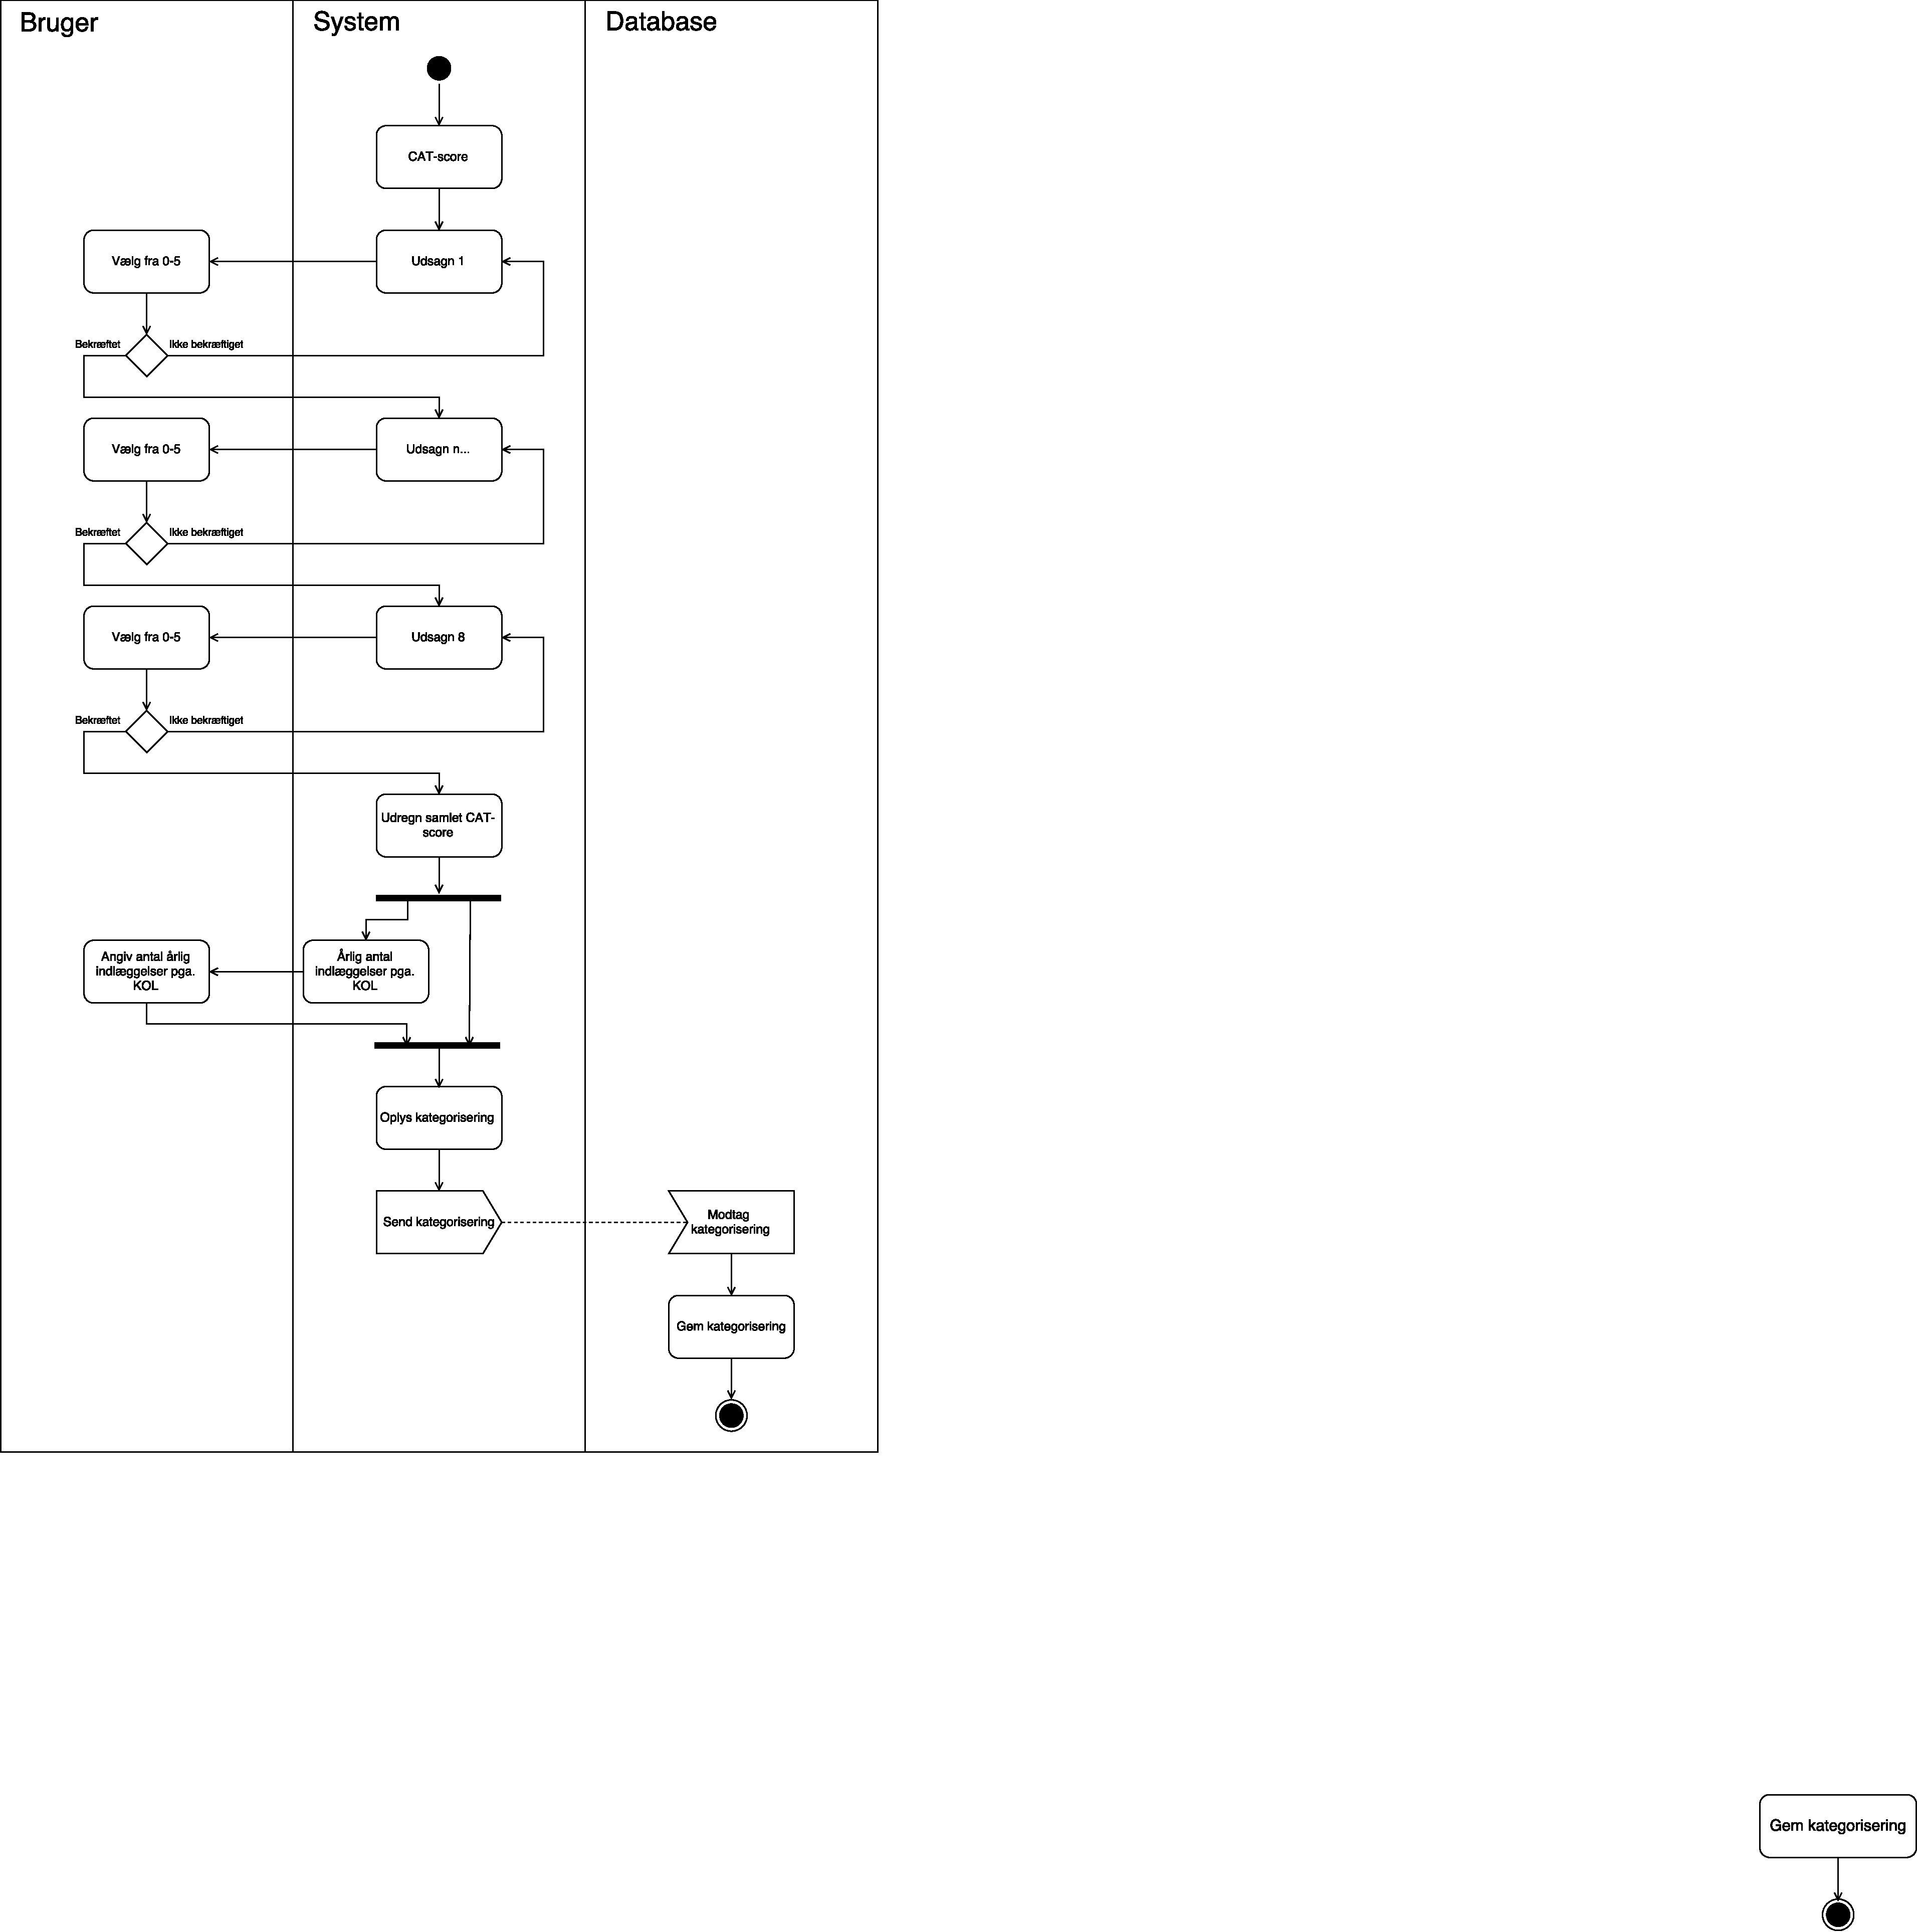
\includegraphics[width=1\textwidth]{figures/aktivitetsdiagram/Kategorisering}
\caption{Aktivitetsdiagram for kategorisering af KOL-patienter.}
\label{fig:Kate}
\end{figure}

\noindent
Systemet starter med at vise en grænseflade for hver af de otte udsagn, der udgør CAT-scoren, jf. \autoref{fig:CAT}. Til hvert af udsagnene angiver brugeren en score passende til deres sygdomstilstand, hvor systemet ud fra de individuelle score beregner en samlet CAT-score. 
Dernæst vises grænsefladen for årlig antal indlæggelser på grund af KOL, hvor brugeren skal angive antal indlæggelser årligt på grund af KOL. Ud fra den samlede CAT-score og antal indlæggelser, beregner systemet brugerens kategorisering af KOL. Efterfølgende viser systemet brugerens kategorisering som  A, B, C eller D.
Kategoriseringen sendes og gemmes i databasen.  